\documentclass{beamer}
\graphicspath{ {graphics/}}
\usepackage[export]{adjustbox}

\begin{document}
\title{Literary Worlds Javascript Client}
\author{Tim Cunningham, John Lewis, Owen Watson}
\usenavigationsymbolstemplate{}
\frame{\titlepage}
\frame{\frametitle{Table of contents}\tableofcontents}

\section{Background}

\frame{\frametitle{Terms and Definitions}
\begin{itemize}
\item MUD - A generic term for a networked, shared virtual environment
\item Server - The MUD "world". A network service which implements the MUD's shared space
\item Client - A program used to connect to a MUD server.
\item Java applet - A small application which is written in Java and can be executed in a web browser
\item Telnet - A network protocol used on the Internet or local area networks to provide an interactive text-oriented communication
\end{itemize}
}

\frame{\frametitle{Background}
\begin{itemize}
  \item Literary Worlds is an MUD used for English education at grade schools
  \item These games are known as MOOs (Multiuser Object Oriented), or MUDs (Multi User Domains)
  \item Many comparable MUDs are text only, and users connect using a telnet client
  \item Literary Worlds uses enCore Xpress which allows the user to browse by clicking links, or by text.
  \item The aim of this project is to provide a drop-in replacement user interface in Javascript
\end{itemize}
}

\frame{\frametitle{Client}
\begin{itemize}
  \item Client: Allen Webb
  \item Professor of Comparative Literature and Postcolonial Studies at Western Michigan University's Department of English
  \item In 2003, Robert Rozema, a PhD student under Allen Webb created the prototype Literary World
  \item The Literary Worlds project was one of seven projects to receive funding from the Western Michigan University President's Innovation Fund
\end{itemize}
}

\frame{\frametitle{Literary Worlds}
  \begin{centering}
  What is a literary world?
  \begin{itemize}
    \item A computer based simulated environment interpreting a literary source text
  \end{itemize}
  \centerline{
  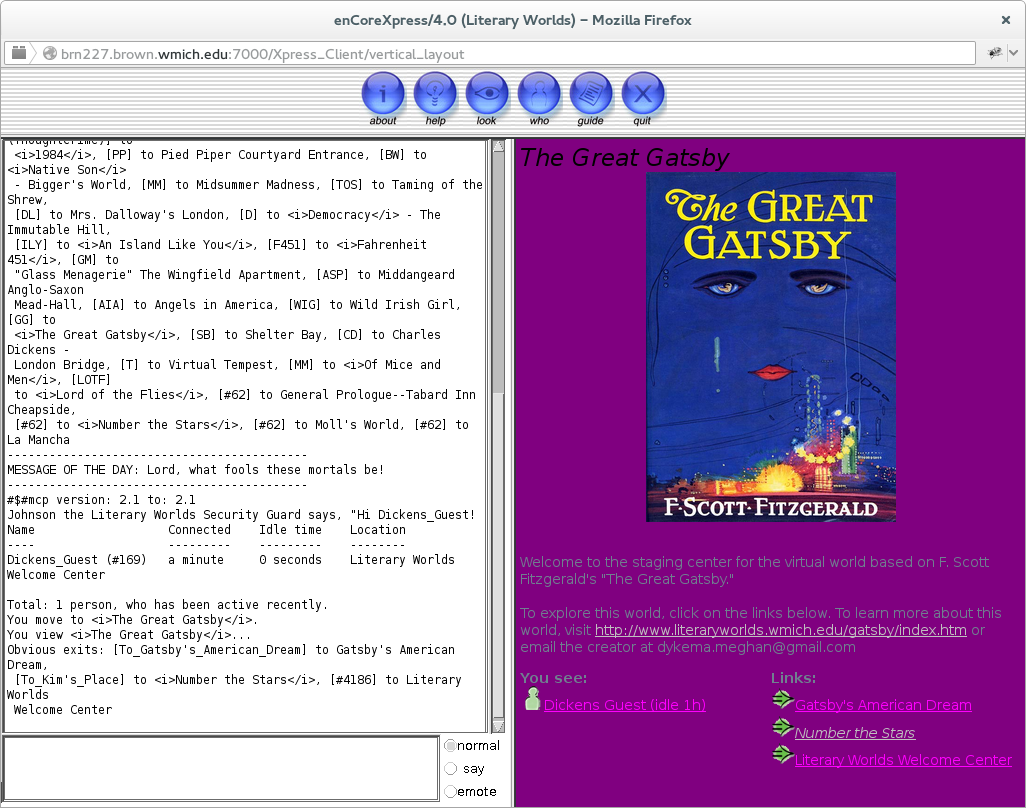
\includegraphics[width=0.75\textwidth,height=\textheight,keepaspectratio]{00_Great_Gatsby_Example.png}}
  \end{centering}
}

\frame{\frametitle{Literary Worlds}
  \begin{centering}
  \begin{itemize}
  \item Within these worlds, users can:
  \begin{itemize}
    \item Interact with characters
    % Both real and virtual (bots)
    \item Manipulate and interact with object
    % Examples given here
    \item Explore virtual environments
  \end{itemize}
  \end{itemize}
  \end{centering}
}

\frame{\frametitle{Example}
  \begin{centering}
  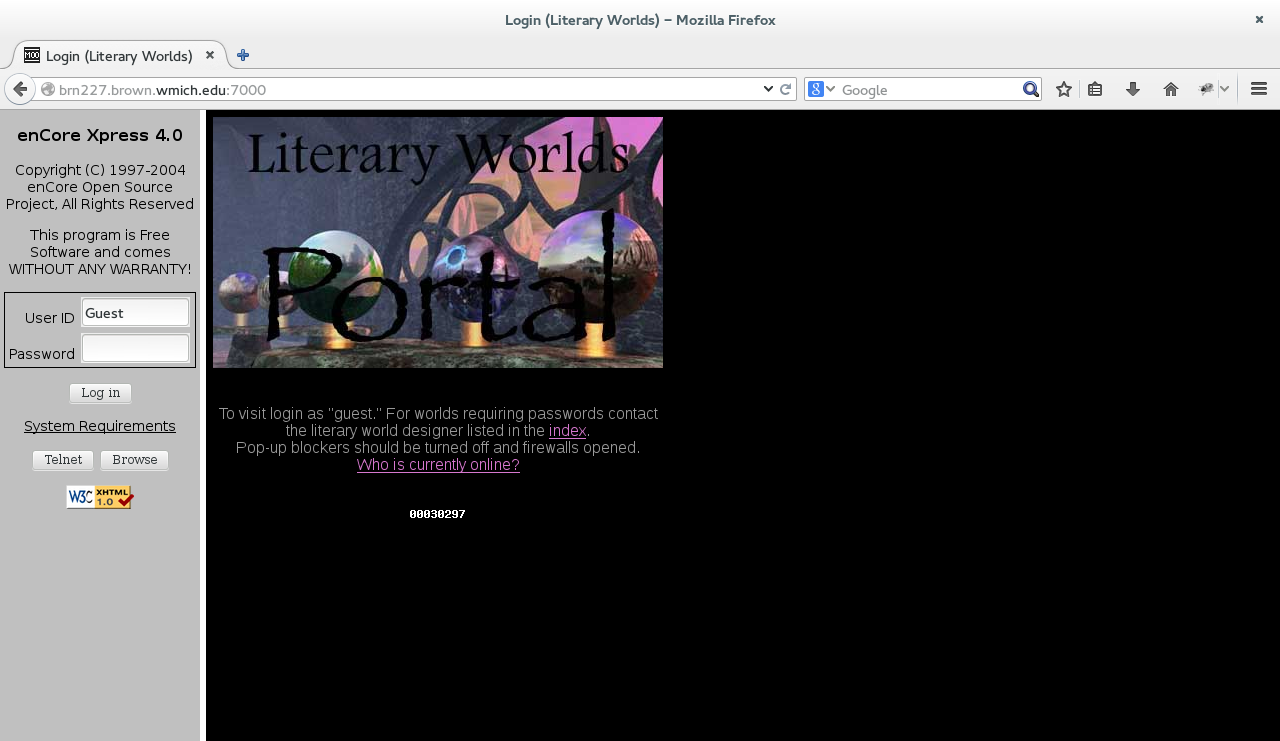
\includegraphics[width=\textwidth,height=\textheight,keepaspectratio]{01_LogIn.png}
  \end{centering}
}

\frame{\frametitle{Example}
  \begin{centering}
  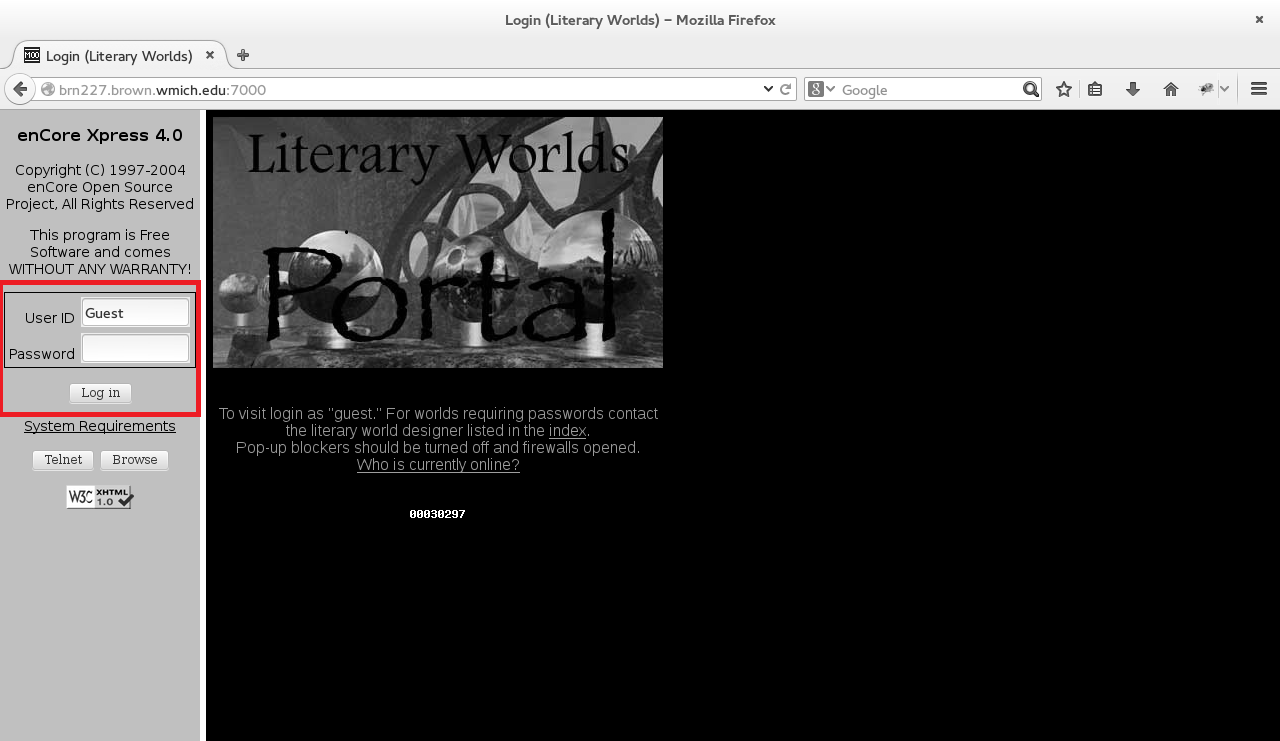
\includegraphics[width=\textwidth,height=\textheight,keepaspectratio]{01_LogIn_GRAY.png}
  \end{centering}
}

\frame{\frametitle{Example}
  \begin{centering}
  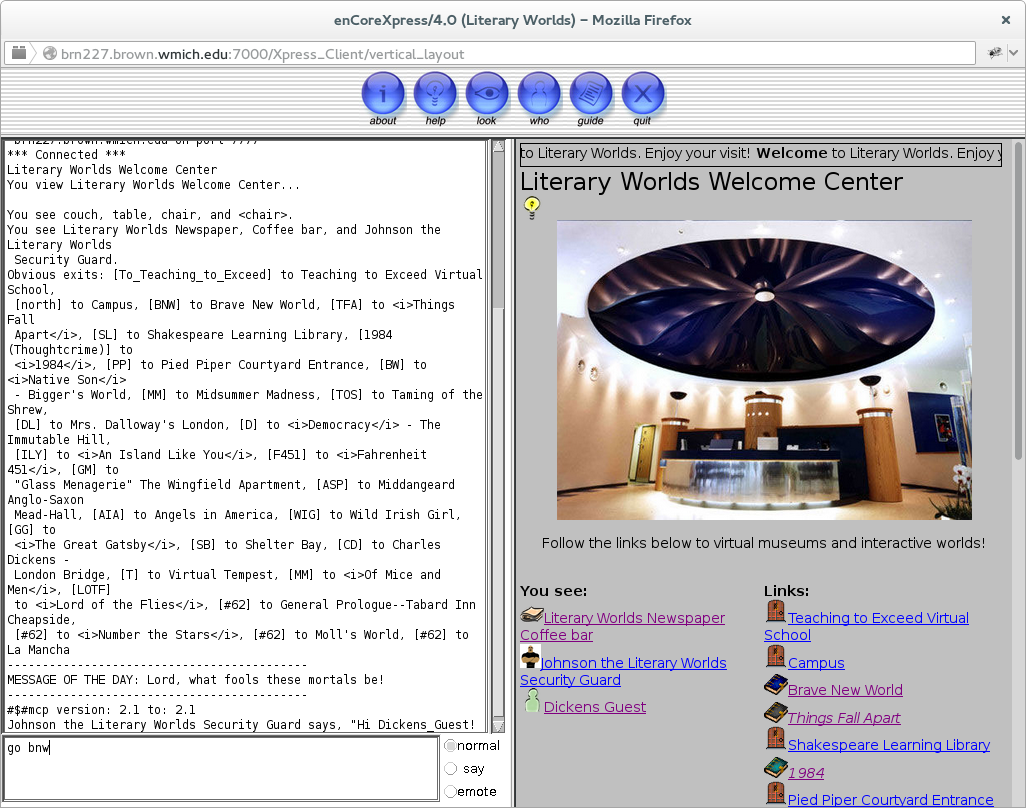
\includegraphics[width=\textwidth,height=\textheight,keepaspectratio]{01_gobnw.png}
  \end{centering}
}

\frame{\frametitle{Example}
  \begin{centering}
  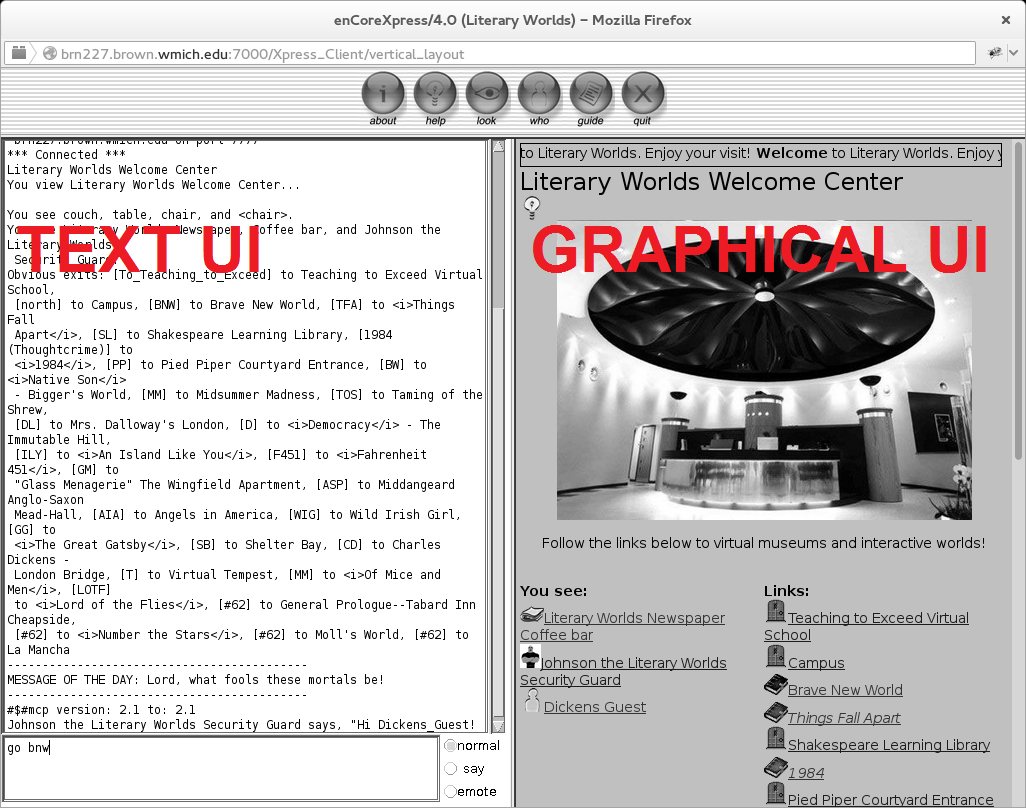
\includegraphics[width=\textwidth,height=\textheight,keepaspectratio]{01_gobnw_ui.png}
  \end{centering}
}

\frame{\frametitle{Example}
  \begin{centering}
  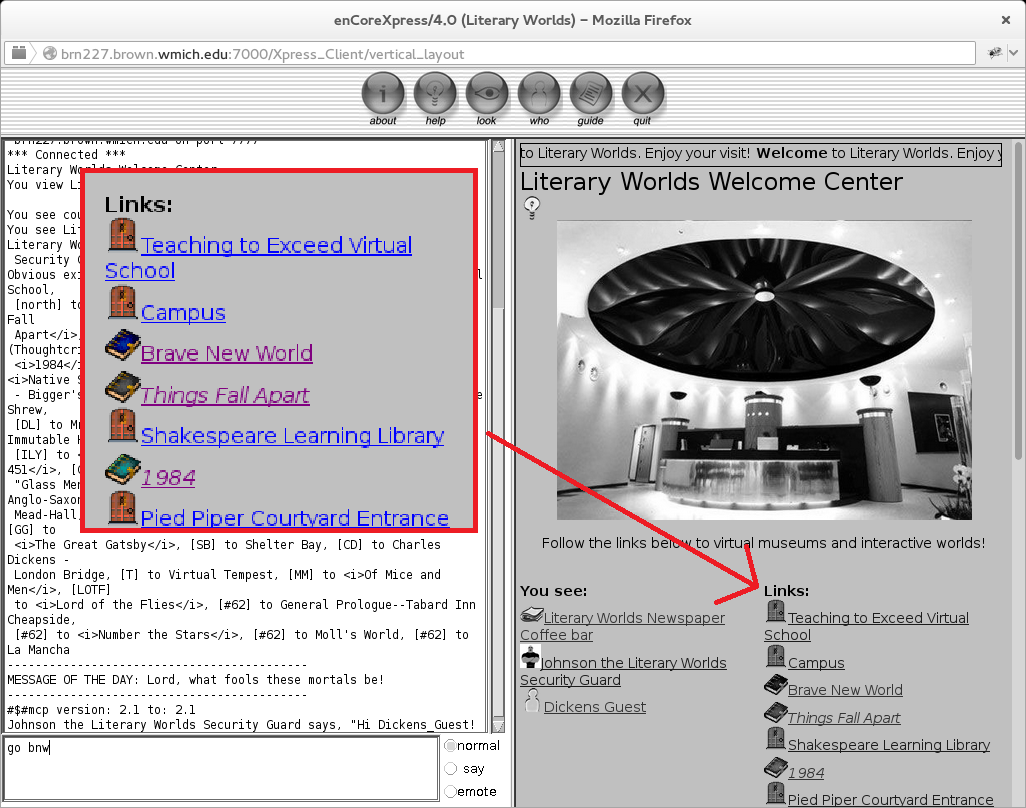
\includegraphics[width=\textwidth,height=\textheight,keepaspectratio]{01_gobnw_Links.png}
  \end{centering}
}

\frame{\frametitle{Example}
  \begin{centering}
  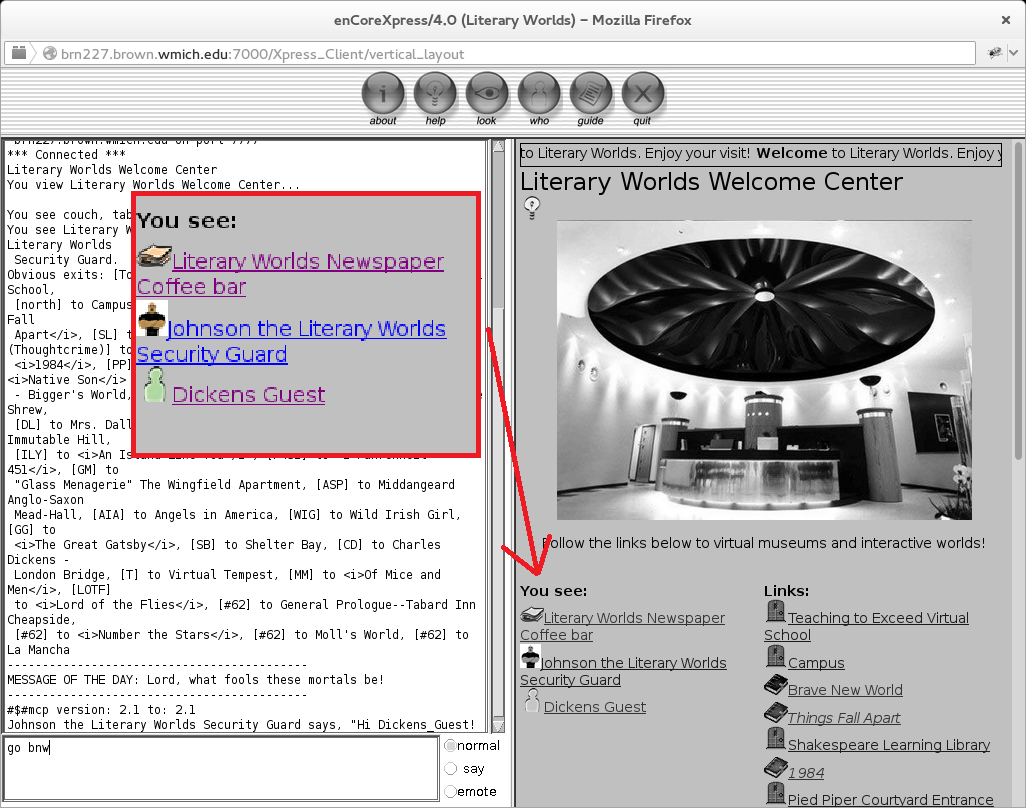
\includegraphics[width=\textwidth,height=\textheight,keepaspectratio]{01_gobnw_Objs.png}
  \end{centering}
}

\frame{\frametitle{Example}
  \begin{centering}
  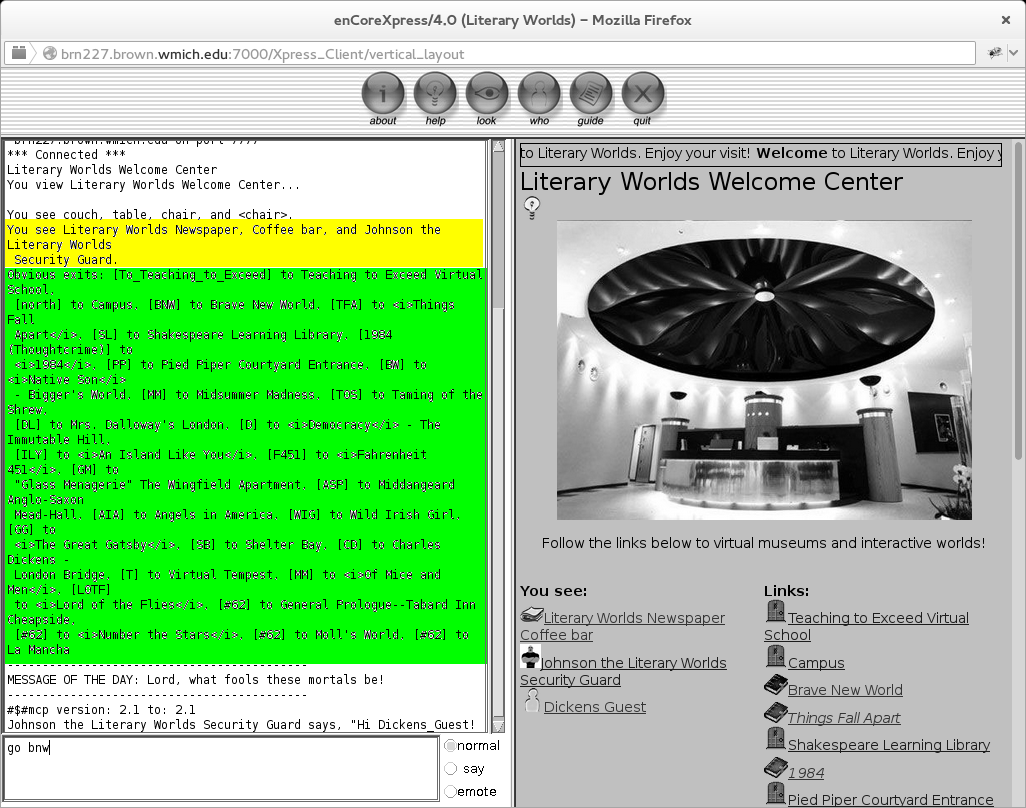
\includegraphics[width=\textwidth,height=\textheight,keepaspectratio]{01_gobnw_telnet.png}
  \end{centering}
}

\frame{\frametitle{Example}
  \begin{centering}
  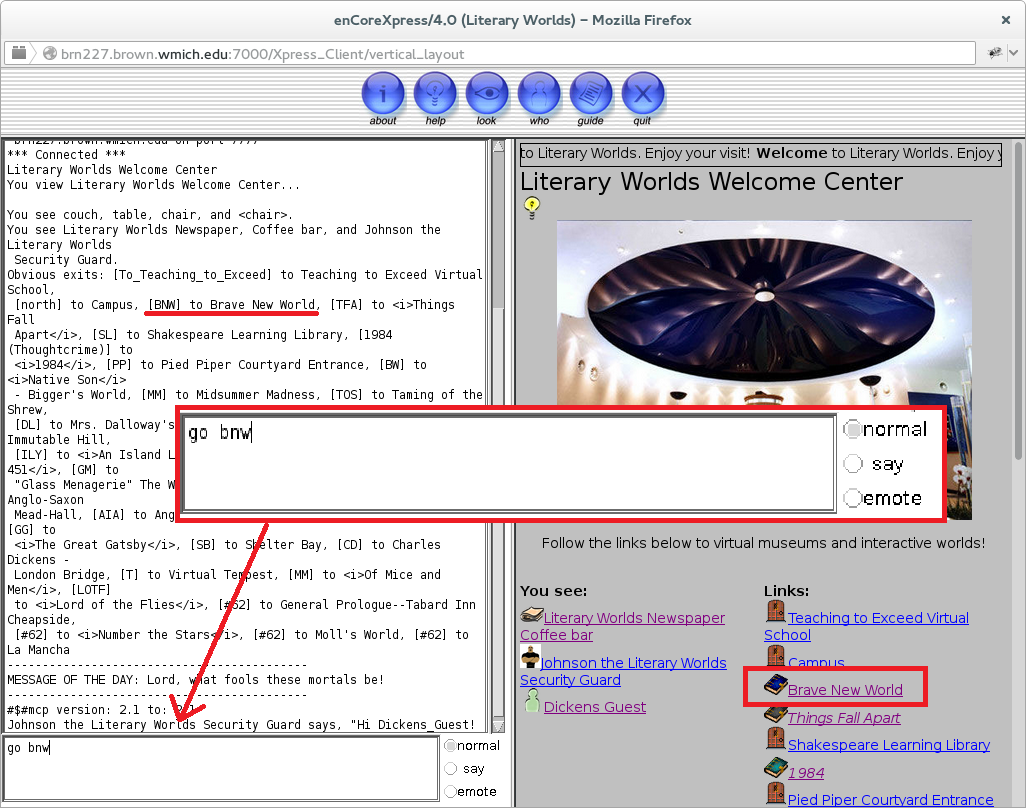
\includegraphics[width=\textwidth,height=\textheight,keepaspectratio]{01_gobnw_cmd.png}
  \end{centering}
}

\frame{\frametitle{Example}
  \begin{centering}
  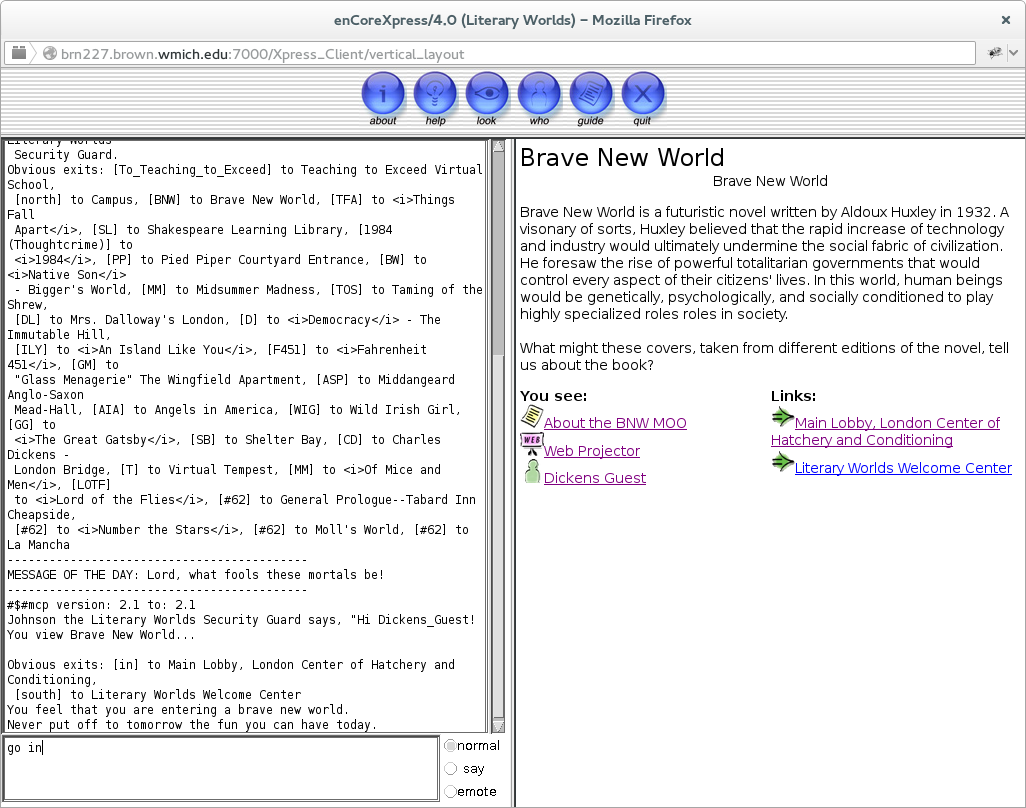
\includegraphics[width=\textwidth,height=\textheight,keepaspectratio]{02_goin.png}
  \end{centering}
}

\frame{\frametitle{Example}
  \begin{centering}
  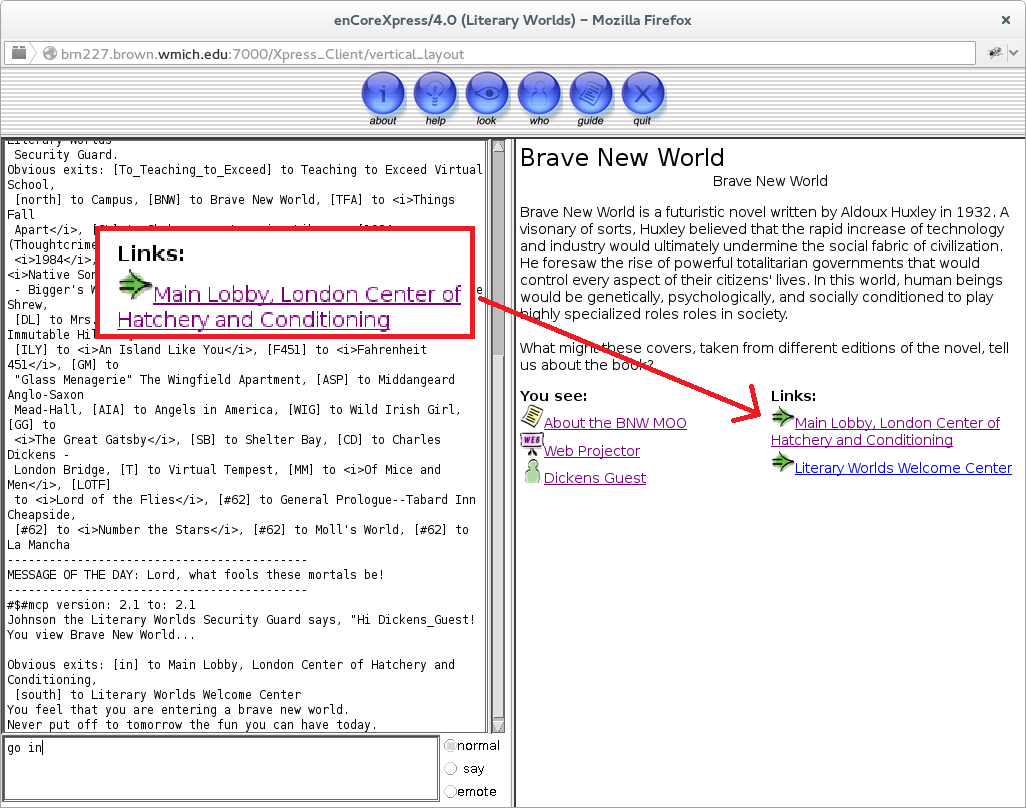
\includegraphics[width=\textwidth,height=\textheight,keepaspectratio]{02_goin_red.png}
  \end{centering}
}

\frame{\frametitle{Example}
  \begin{centering}
  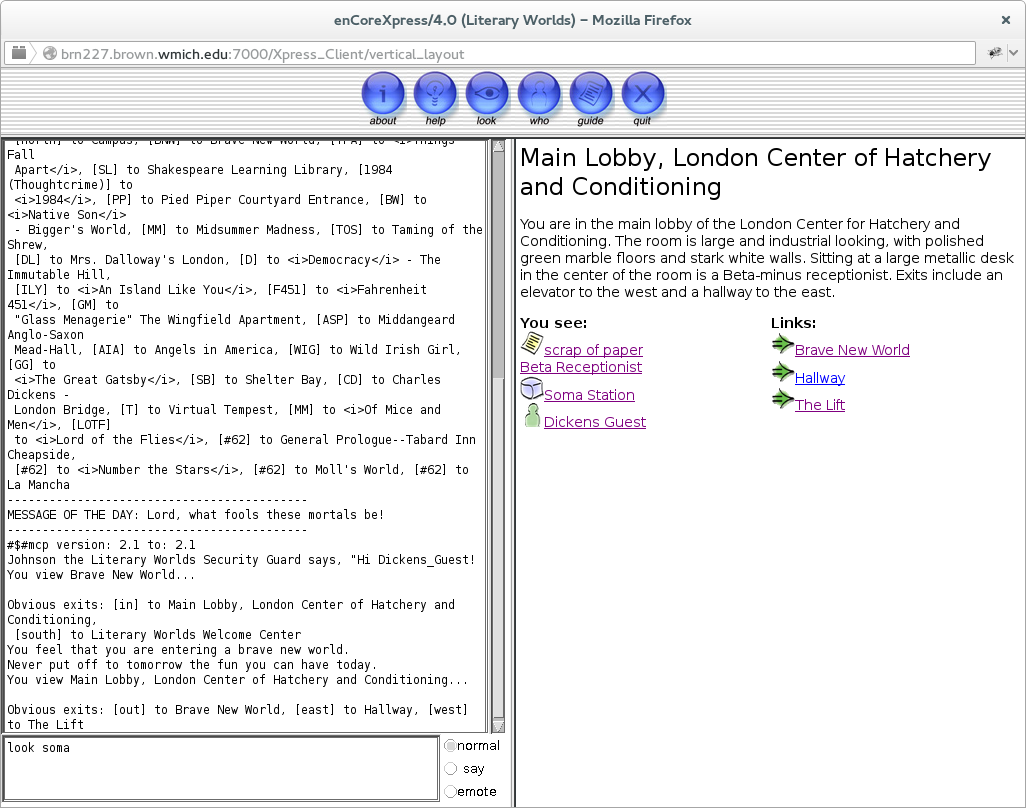
\includegraphics[width=\textwidth,height=\textheight,keepaspectratio]{03_looksoma.png}
  \end{centering}
}

\frame{\frametitle{Example}
  \begin{centering}
  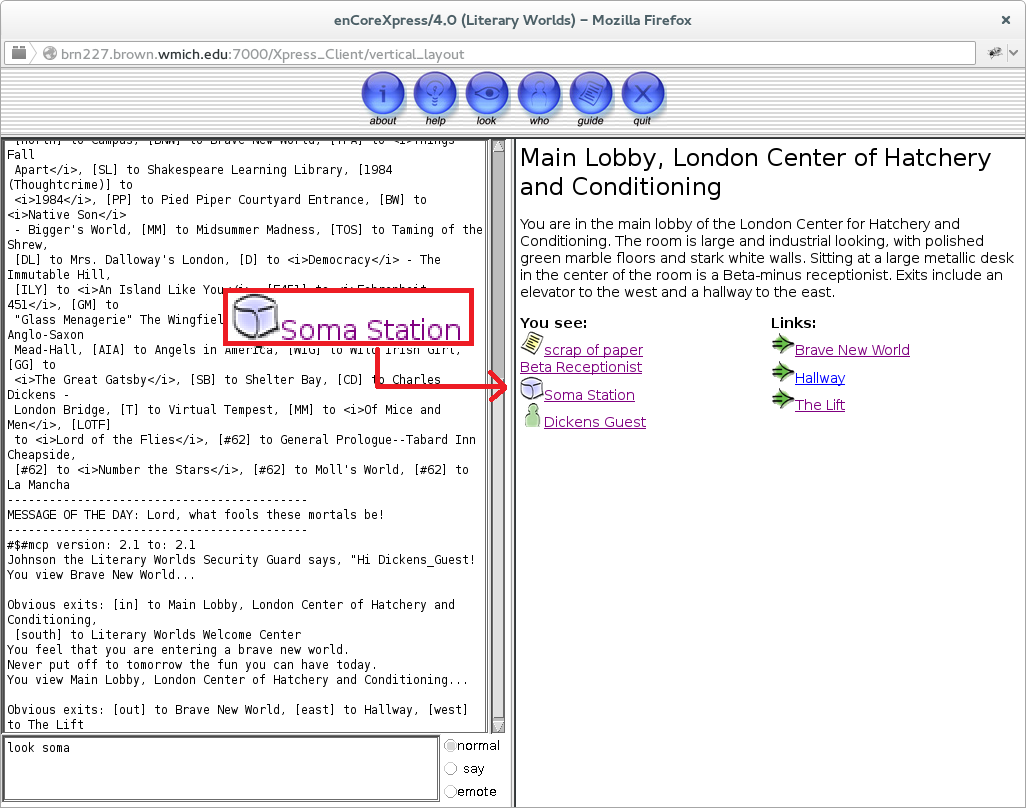
\includegraphics[width=\textwidth,height=\textheight,keepaspectratio]{03_looksoma_red.png}
  \end{centering}
}

\frame{\frametitle{Example}
  \begin{centering}
  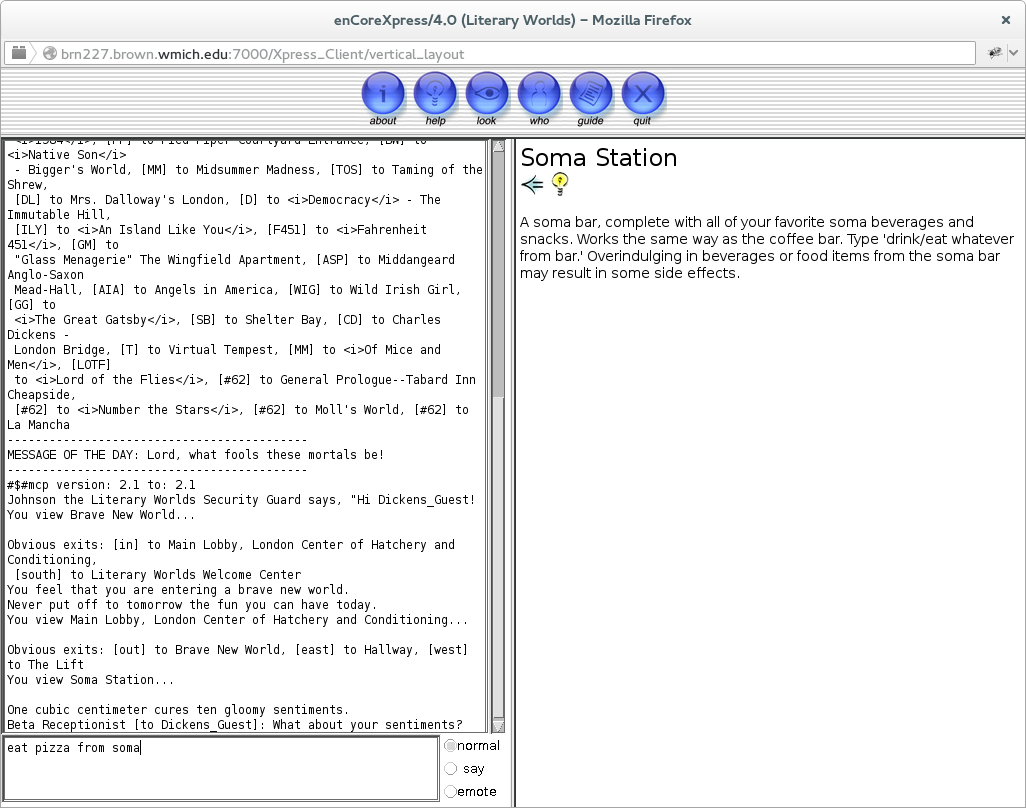
\includegraphics[width=\textwidth,height=\textheight,keepaspectratio]{04_eatpizzafromsoma.png}
  \end{centering}
}

\frame{\frametitle{Example}
  \begin{centering}
  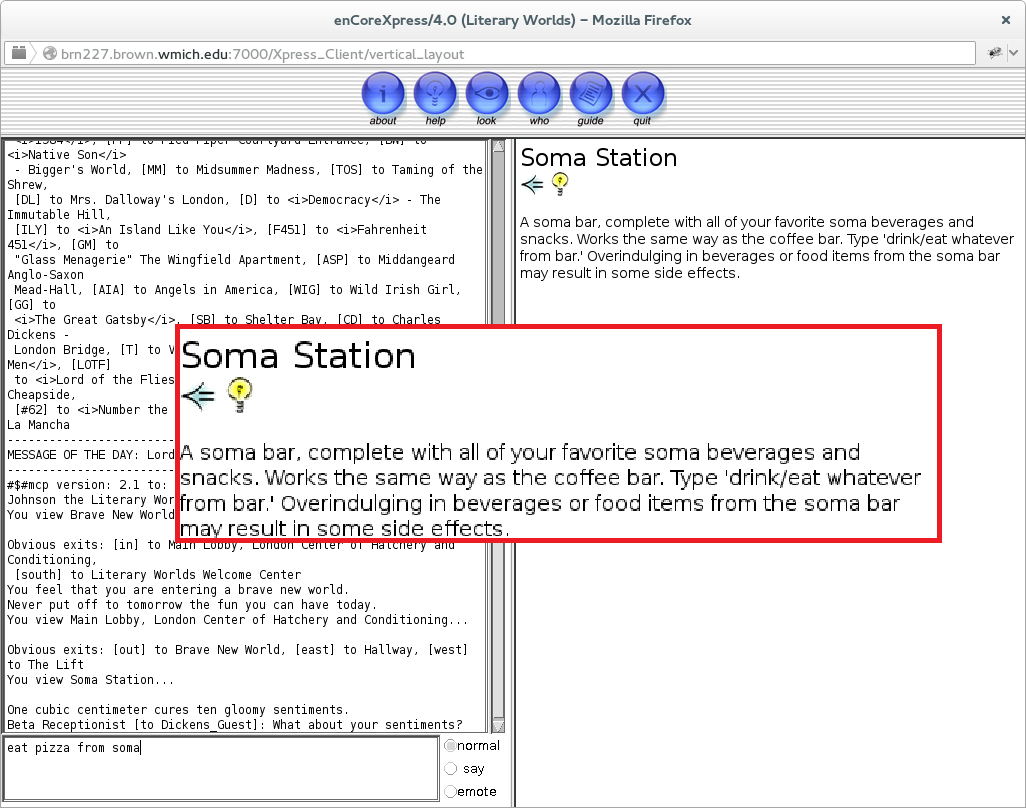
\includegraphics[width=\textwidth,height=\textheight,keepaspectratio]{04_eatpizzafromsoma_red1.png}
  \end{centering}
}

\frame{\frametitle{Example}
  \begin{centering}
  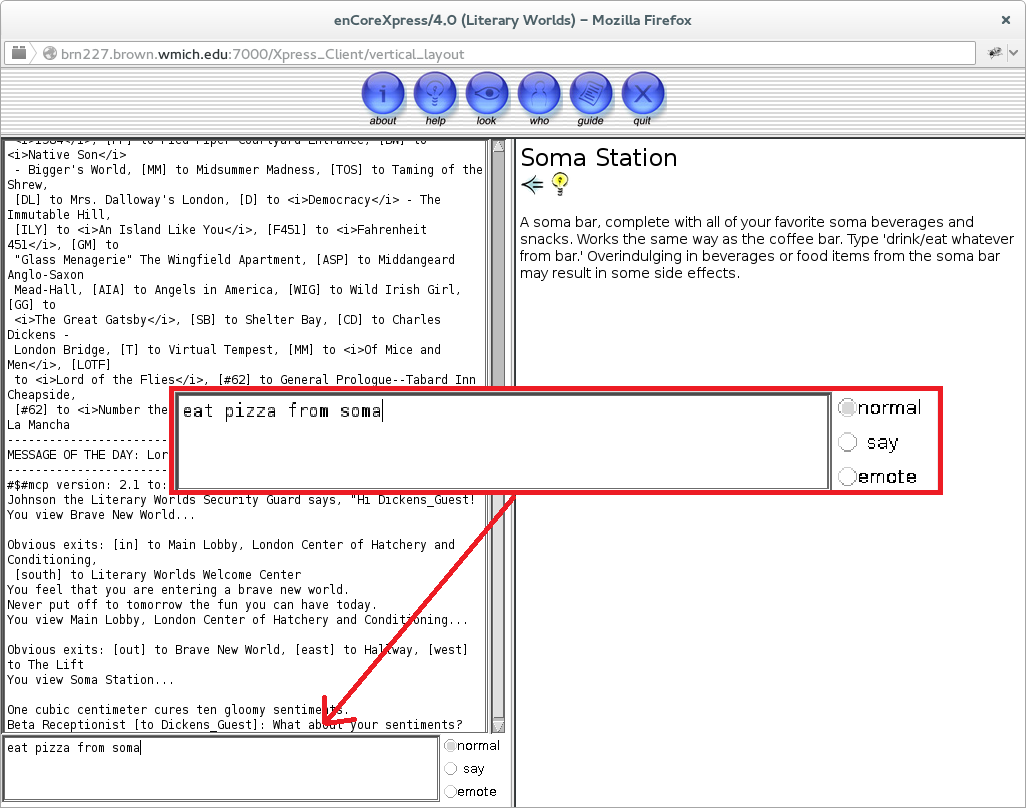
\includegraphics[width=\textwidth,height=\textheight,keepaspectratio]{04_eatpizzafromsoma_red2.png}
  \end{centering}
}

\frame{\frametitle{Example}
  \begin{centering}
  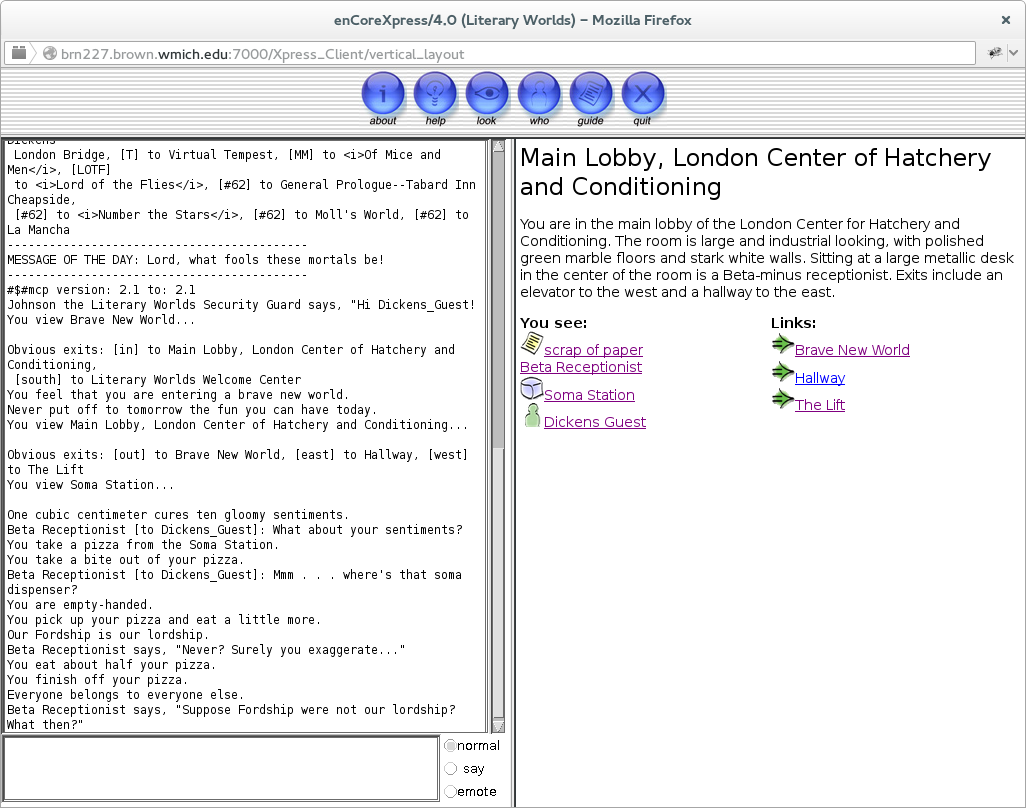
\includegraphics[width=\textwidth,height=\textheight,keepaspectratio]{06_pizzadone.png}
  \end{centering}
}

\frame{\frametitle{Example}
  \begin{centering}
  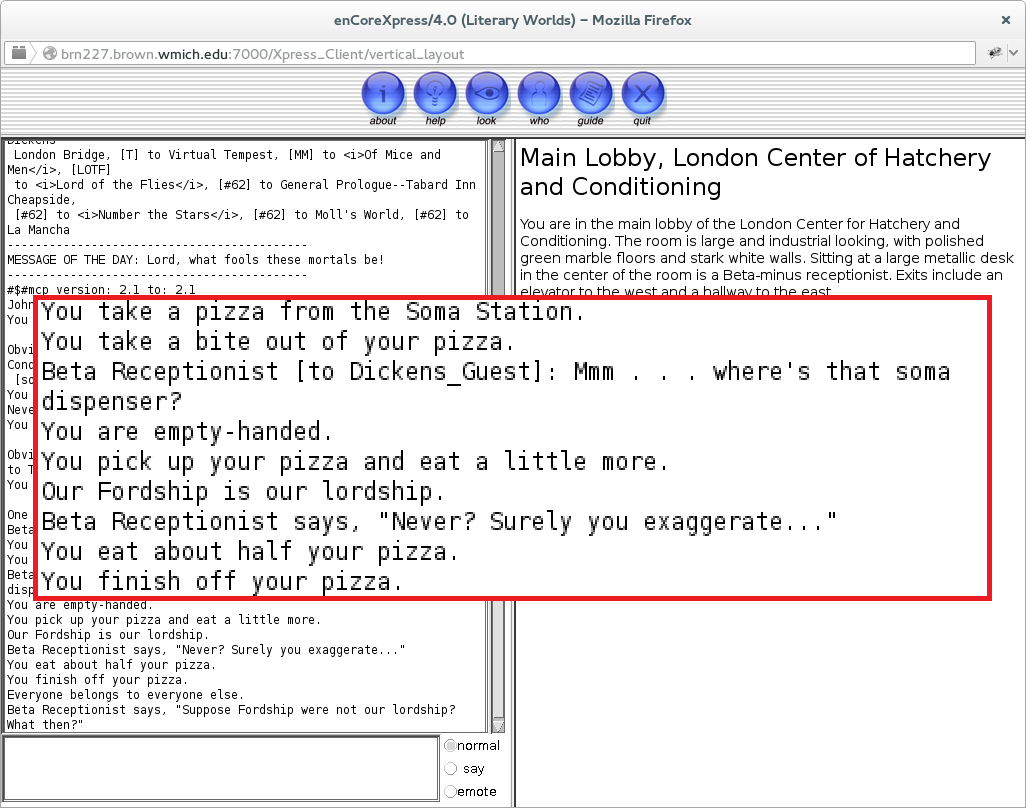
\includegraphics[width=\textwidth,height=\textheight,keepaspectratio]{06_pizzadone_red.png}
  \end{centering}
}

\frame{\frametitle{Example}
  \begin{centering}
  GUI only and Text only modes are available
  
  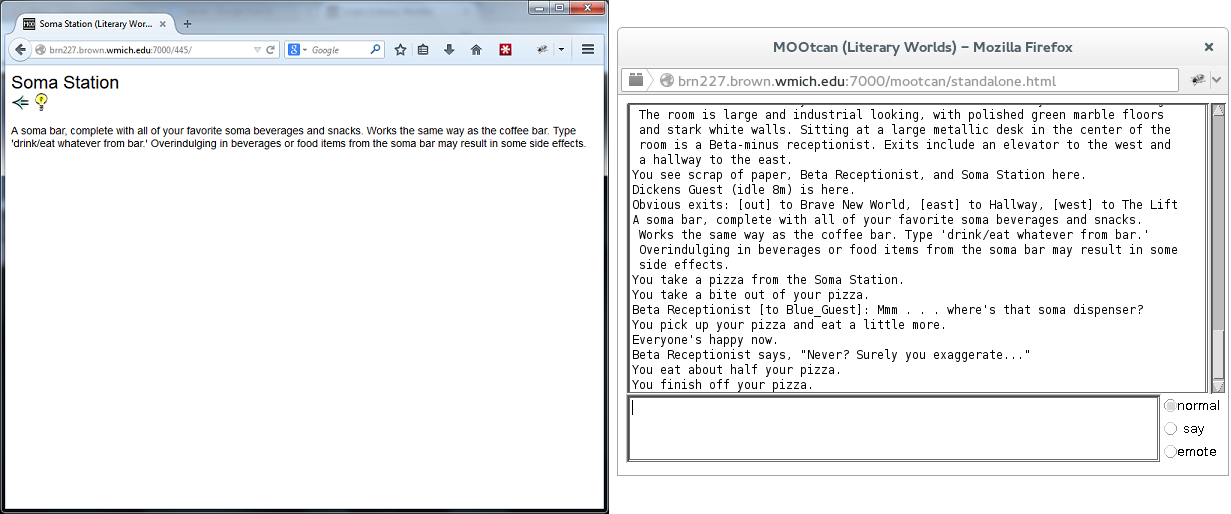
\includegraphics[width=\textwidth,height=\textheight,keepaspectratio]{GUInTUIOnly.png}
  \end{centering}
}

\frame{\frametitle{Only The Basics}
  \begin{centering}
  Literary Worlds can also be used for more than one user
  \begin{itemize}
    \item Entire classrooms with many users
    \item Log on a characters from the text
    \item Village of Umofia created by Dr. Allen Webb
  \end{itemize}
   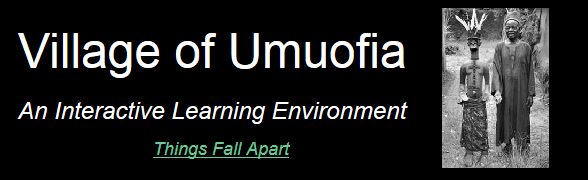
\includegraphics[width=\textwidth,height=\textheight,keepaspectratio]{vou_logo.png}
  \end{centering}
}

\frame{\frametitle{More Literary World Examples}
\begin{centering}
Village of Umuofia 
\begin{itemize}
\item Users may use this environment in a variety of ways
\begin{itemize}
\item A gallery of images of Igbo village that show life and traditional West African music
\item An interactive space for live action role play activities based on the novel (Things Fall Apart)
\end{itemize}
\end{itemize}
\end{centering}
}

\frame{\frametitle{More Literary World Examples}
\begin{centering}
Village of Umuofia
\begin{itemize}
\item Literary Worlds allows users to further understand the novel's characters, environments, and themes
\end{itemize}
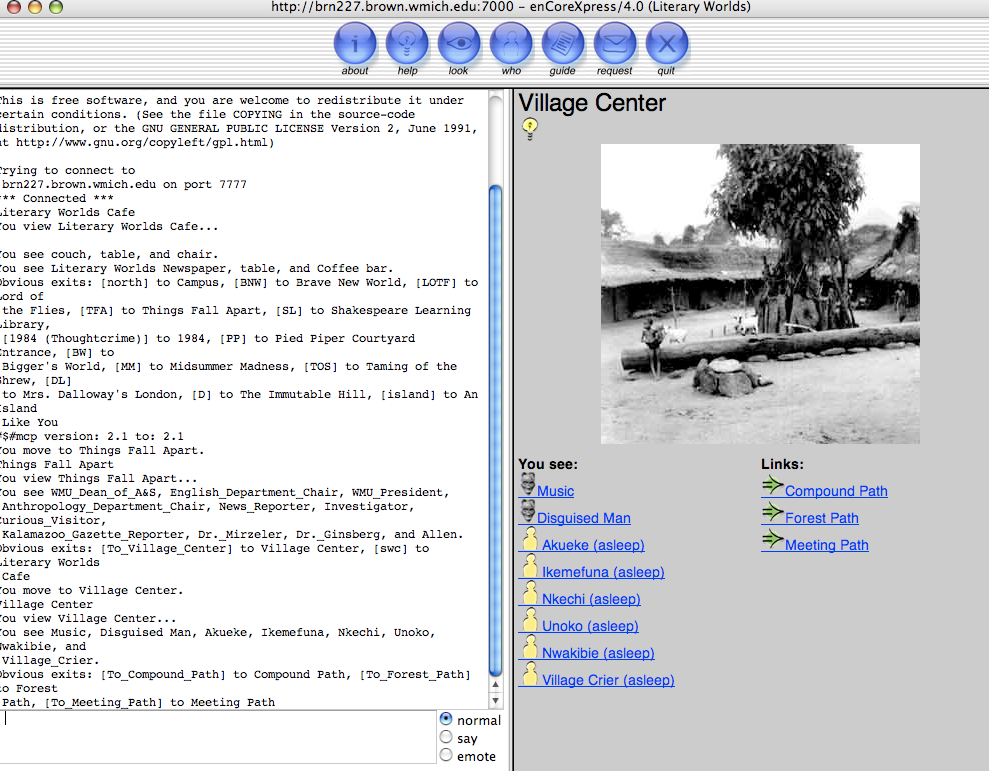
\includegraphics[width=0.75\textwidth,height=\textheight,keepaspectratio,center]{village.png}
\end{centering}
}

\section{Introduction}

\frame{\frametitle{Current Technology}
  \begin{itemize}
    \item LambdaMOO - A MUD server software package
    %\item LambdaMOO is distributed as a source tarball, deploying it on a new sever entails compiling it, and running it using the enCore database, and configuring Apache to work with enCore.
    \item enCore Xpress is an graphical interface and MUD database package that works with the LambdaMOO server to provide a browser based text client using a Java applet as well as a graphical, mouse driven interface.
    %\item The Java applet is the text interface, it makes a telnet to LambdaMOO, as though the user were using a command line telnet client.
    \item Literary Worlds uses version 4 of enCore
  \end{itemize}
}

\frame{\frametitle{Current Technology}
  \centerline{
  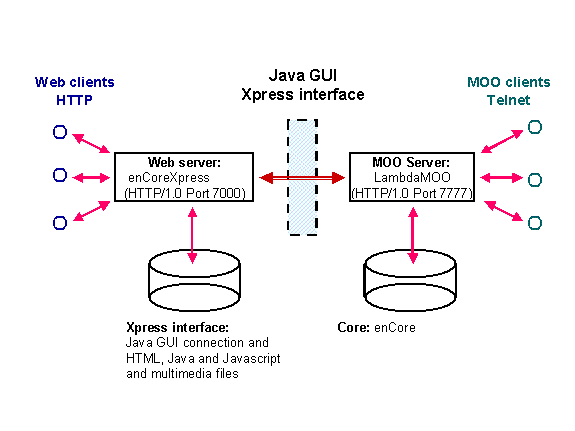
\includegraphics[width=\textwidth,height=\textheight,keepaspectratio]{Xpress_Model.png}}

}

\frame{\frametitle{Problems}
  \begin{centering}
  The current Literary Worlds portal requires:
  \begin{itemize}
  \item Pop-up windows to be allowed
  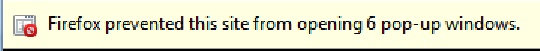
\includegraphics[width=0.8\textwidth,height=\textheight,keepaspectratio]{popupban.png}
  \item Java Runtime Environment (JRE)
  \end{itemize}
  \centerline{
  
\includegraphics[width=0.1\textwidth,height=\textheight,keepaspectratio]{Java_logo.png}}
  \end{centering}
}

\frame{\frametitle{Problems - Java}
  \begin{centering}
  Java Runtime Environment
  \begin{itemize}
  \item It requires the JRE to be installed on all client computers
  \end{itemize}
  \centerline{
  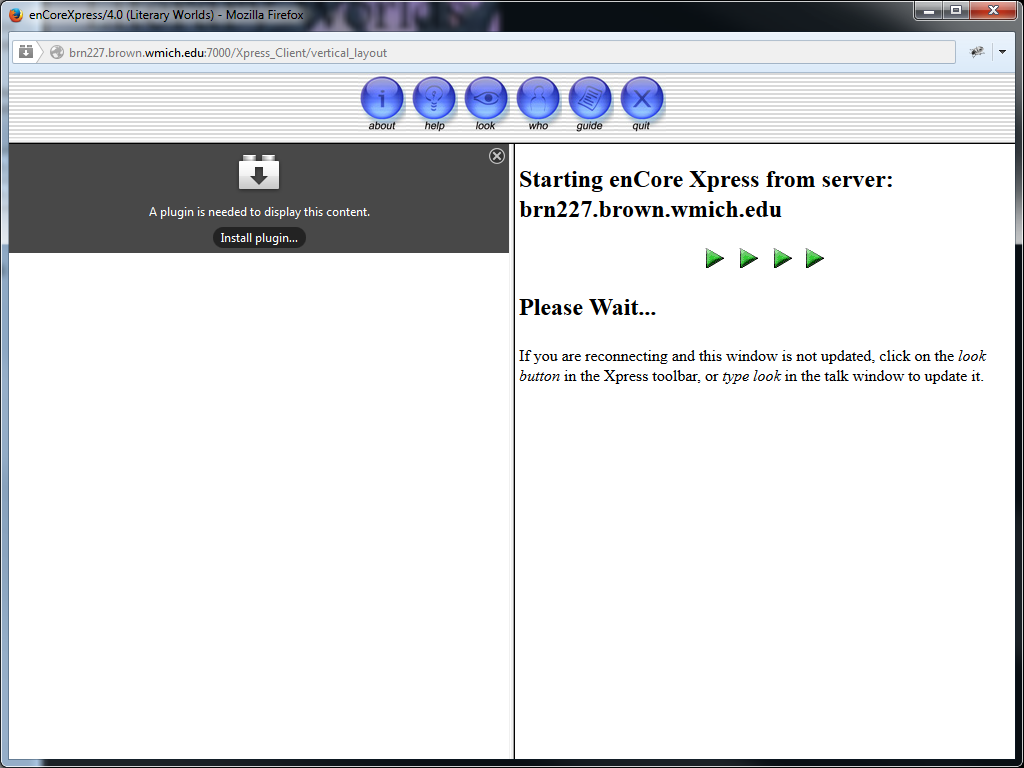
\includegraphics[width=\textwidth,height=0.8\textheight,keepaspectratio]{PlugInNeeded.png}}
  \end{centering}
}

\frame{\frametitle{Problems - Java}
  \begin{centering}
  Java applets in browsers can be difficult
  \begin{itemize}
  \item Java is beginning to be blocked by default in the browser
  \end{itemize}
  \centerline{
  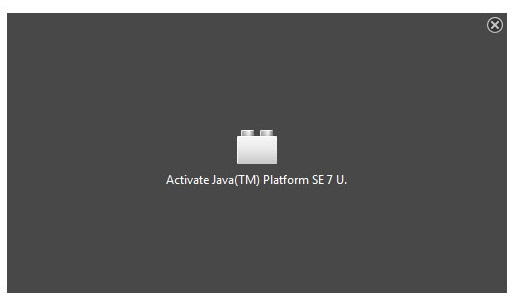
\includegraphics[width=\textwidth,height=\textheight,keepaspectratio]{activatejava.jpg}}
  \end{centering}
}

\frame{\frametitle{Problems - Java}
  \begin{centering}
  Java permissions
  \begin{itemize}
  \item All Java applets do not run without permission from the user
  \item Java requires constant updates due to security concerns
  \end{itemize}
  \centerline{
  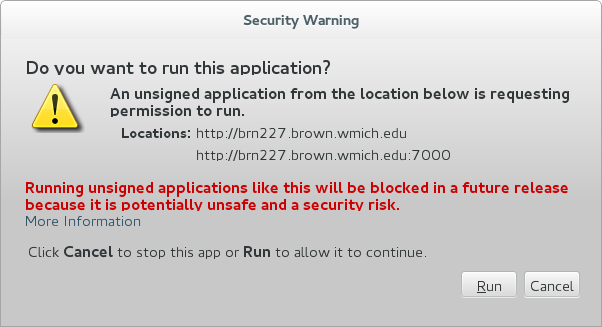
\includegraphics[width=\textwidth,height=\textheight,keepaspectratio]{javasecr.png}}
  \end{centering}
}

\frame{\frametitle{Things to Keep in Mind}
  \begin{centering}
  Over 20 virtual worlds currently make up Literary Worlds
  \begin{itemize}
  \item Any replacement interface needs to keep the virtual worlds functioning, as they are.
    \begin{itemize}
    \item No change to the current server
    \end{itemize}
  \item Need to remove the Java dependency
  \item Need to remove the use of pop ups
  \end{itemize}
  \end{centering}
}

\frame{\frametitle{Current Client-Server Diagram}
  \begin{centering}
  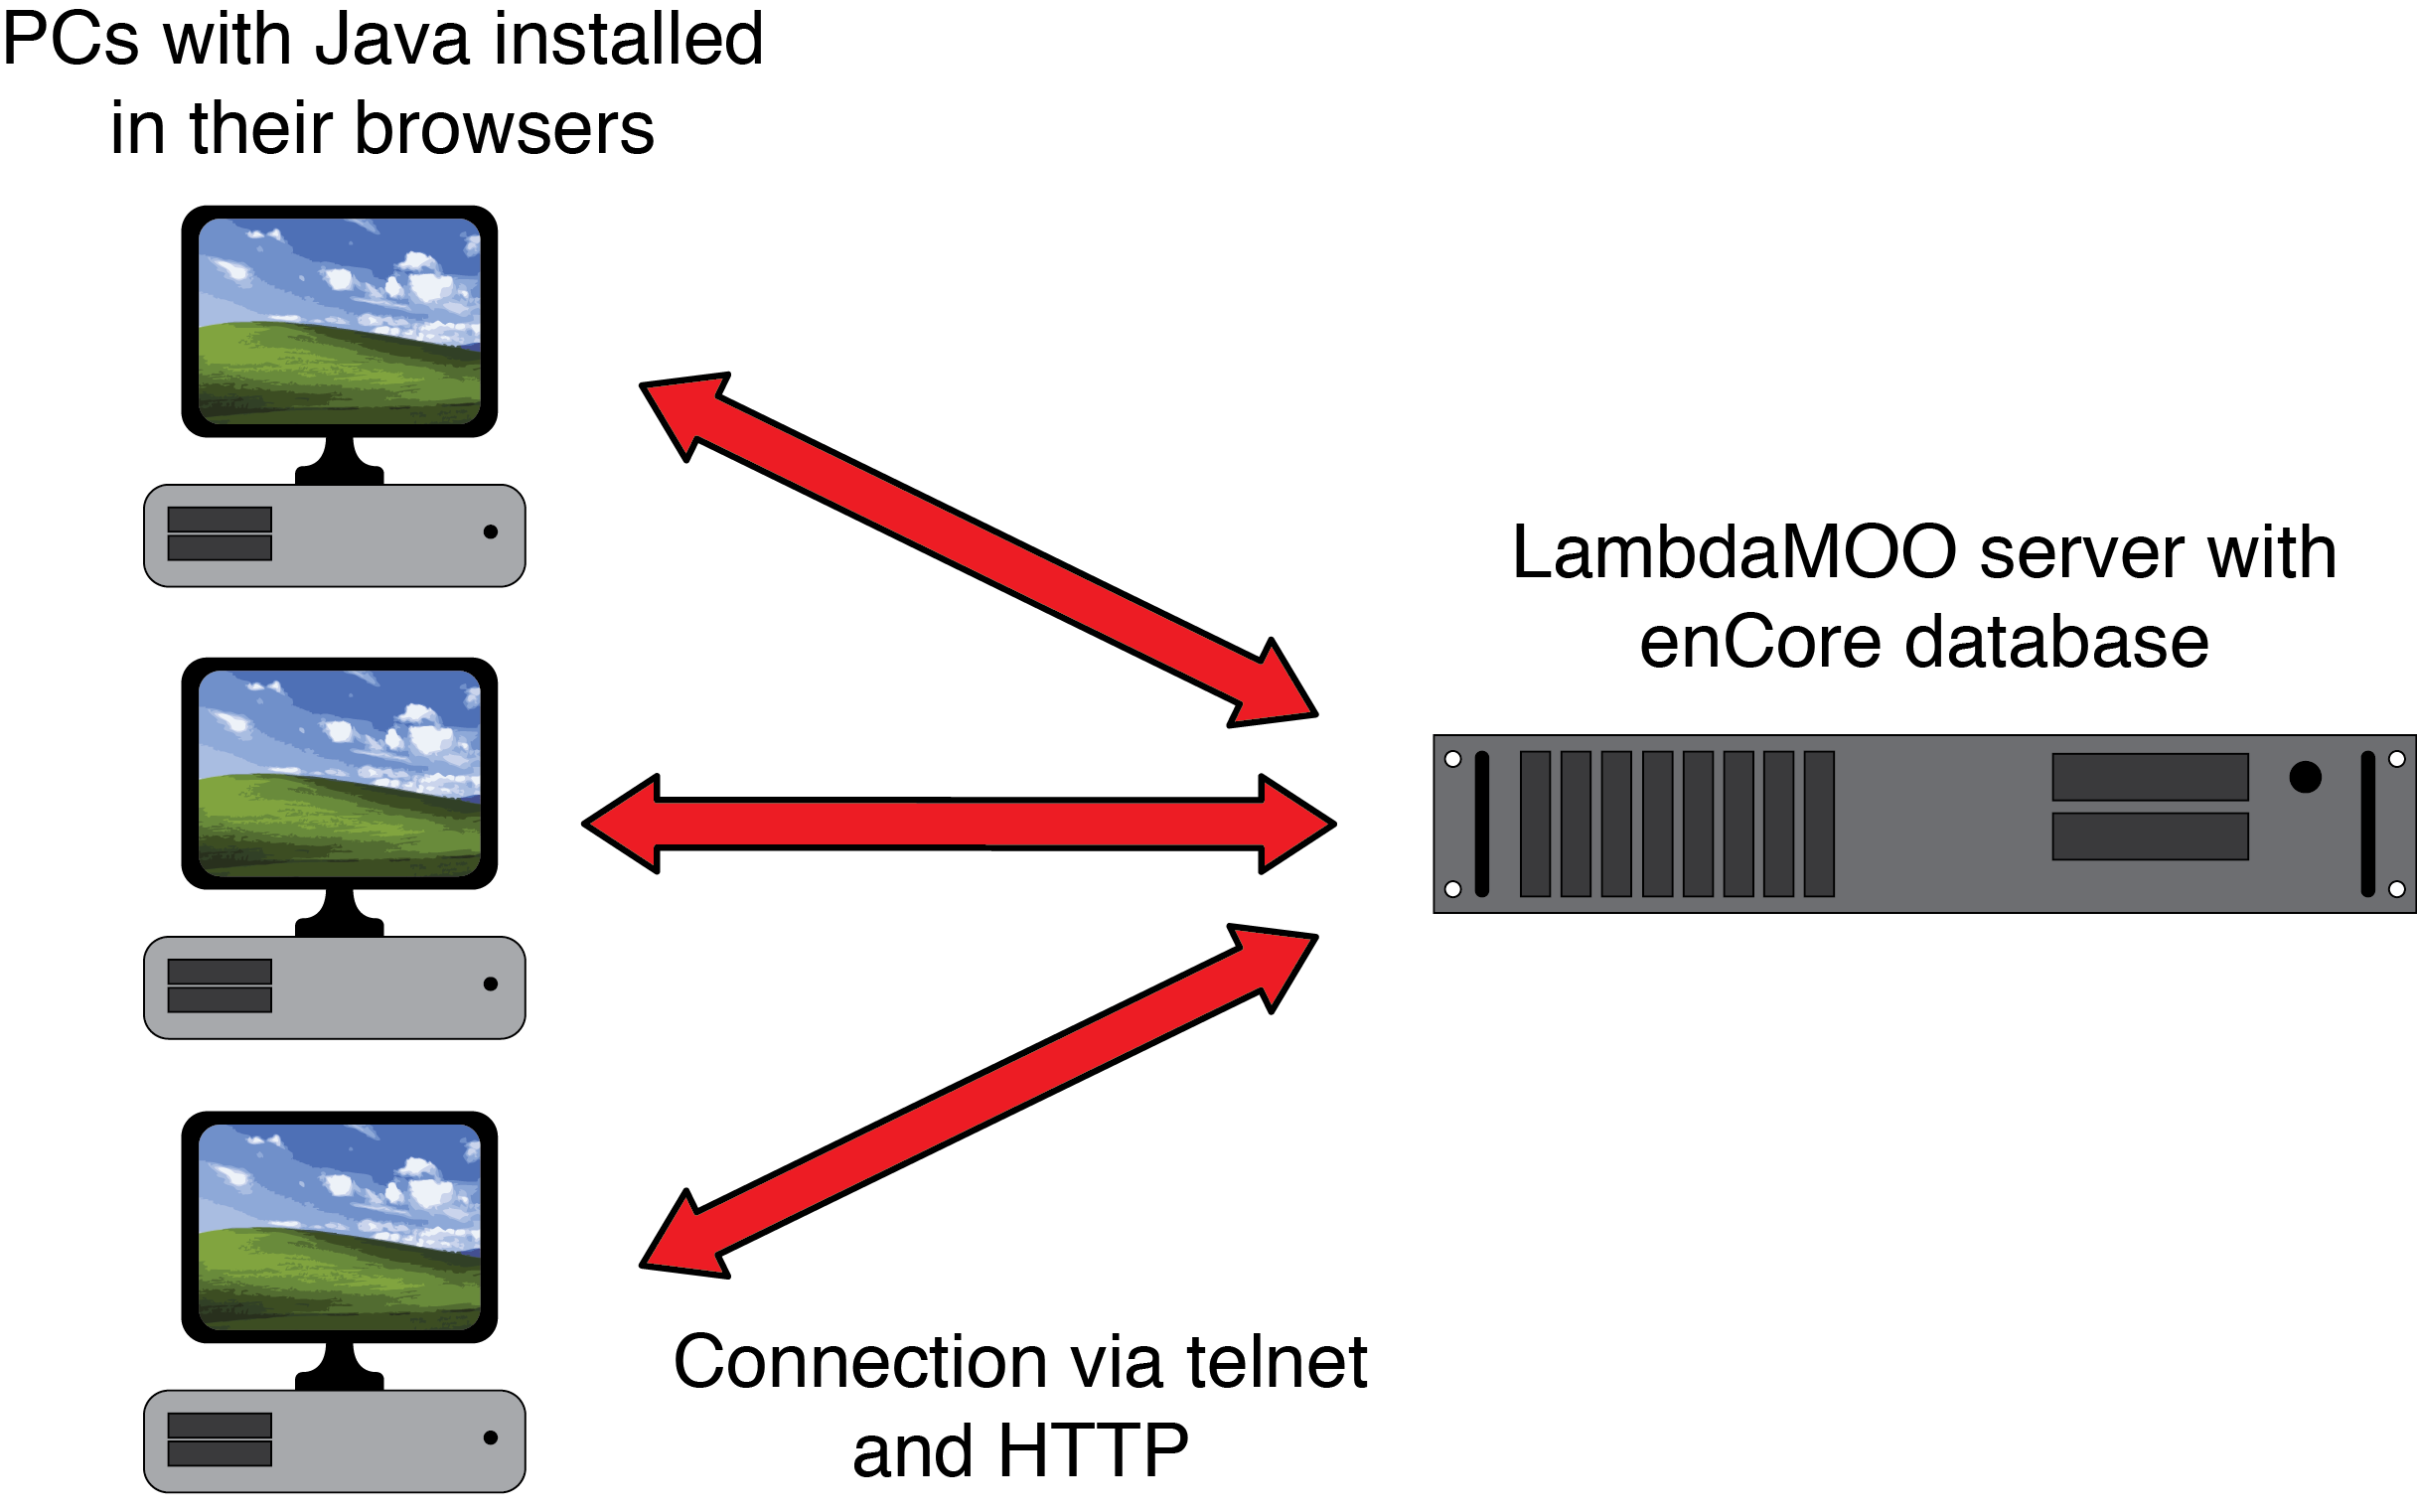
\includegraphics[width=\textwidth,height=\textheight,keepaspectratio]{TelnetDiagram.png}
  \end{centering}
}

\section{Design Decisions}
\frame{\frametitle{New Client-Server Design}
  \begin{itemize}
    \item It is not possible to initiate a raw TCP connection in clientside Javascript, unlike Java applets.

    \item Therefore, we need an intermediary server to connect over TCP, as well as to the browser client, and send data back and forth between the two.

    \item This server must also support multiple concurrent users and handle asynchronous tasks and events.
    \item The new interface must also keep the graphical and text modes in sync as the user moves.
  \end{itemize}
}

\frame{\frametitle{Design Decisions}
  \begin{itemize}
  \item Text Mode
    \begin{itemize}
      \item Client side Javascript MUD client
      \item This is reason an intermediary server is needed, to handle the telnet connection on behalf of each client.
    \end{itemize}
  \item Graphical Mode
    \begin{itemize}
      \item This work is already done in enCore Xpress, there is no need to reinvent it.
      \item The new web application will simply need to serve the existing enCore Xpress interface in a coherent way.
    \end{itemize}
  \end{itemize}
}

\frame{\frametitle{New Client Technology}
  % Backbone, Bootstrap, Socket.io, Coffeescript
  
\includegraphics[width=\textwidth, height=\textheight,keepaspectratio]{clientstack.png}
  \begin{itemize}
  \item Socket.io
    \begin{itemize}
      \item Allows realtime communication between a server program and browser clients.
    \end{itemize}
  \item Backbone
    \begin{itemize}
      \item Backbone is a templating library for Javascript web applications
    \end{itemize}
  \item Bootstrap
    \begin{itemize}
    \item Bootstrap is a frontend layout toolkit
    \end{itemize}
  \item Coffeescript
    \begin{itemize}
      \item Coffeescript is a simple language that translates to Javascript
    \end{itemize}
  \end{itemize}
}

\frame{\frametitle{New Client Alternatives}
%What didn't we use and why - Client
TBD - List of other technologies we did not use.
}

\frame{\frametitle{Intermediate Server Technology}
  % Node.JS here
  
\includegraphics[width=0.66\textwidth, height=\textheight,keepaspectratio,center]{serverstack.png}
  \begin{itemize}
  \item Node.js
    \begin{itemize}
      \item Node.js is a server side runtime that uses the asynchronous features of Javascript to build web application servers. It provides a rich set of networking libraries, and uses the Google Chrome Javascript engine, V8.
      \item It is the first class citizen for socket.io, so it was natural to choose it for the server.
    \end{itemize}
  \item Express
    \begin{itemize}
      \item Express is a web app framework for Node.js
      \item In provides tools such as easy interfaces for REST, URL routing, cookies, etc. similar to what Ruby on Rails does for the Ruby language.
    \end{itemize}
    \item Socket.io
  \end{itemize}
}

\frame{\frametitle{Intermediate Server Alternatives}
%What didn't we use and why - Server
TBD - More things we didn't use and why.
}

\frame{\frametitle{New Client-Server Diagram}
  \begin{centering}
  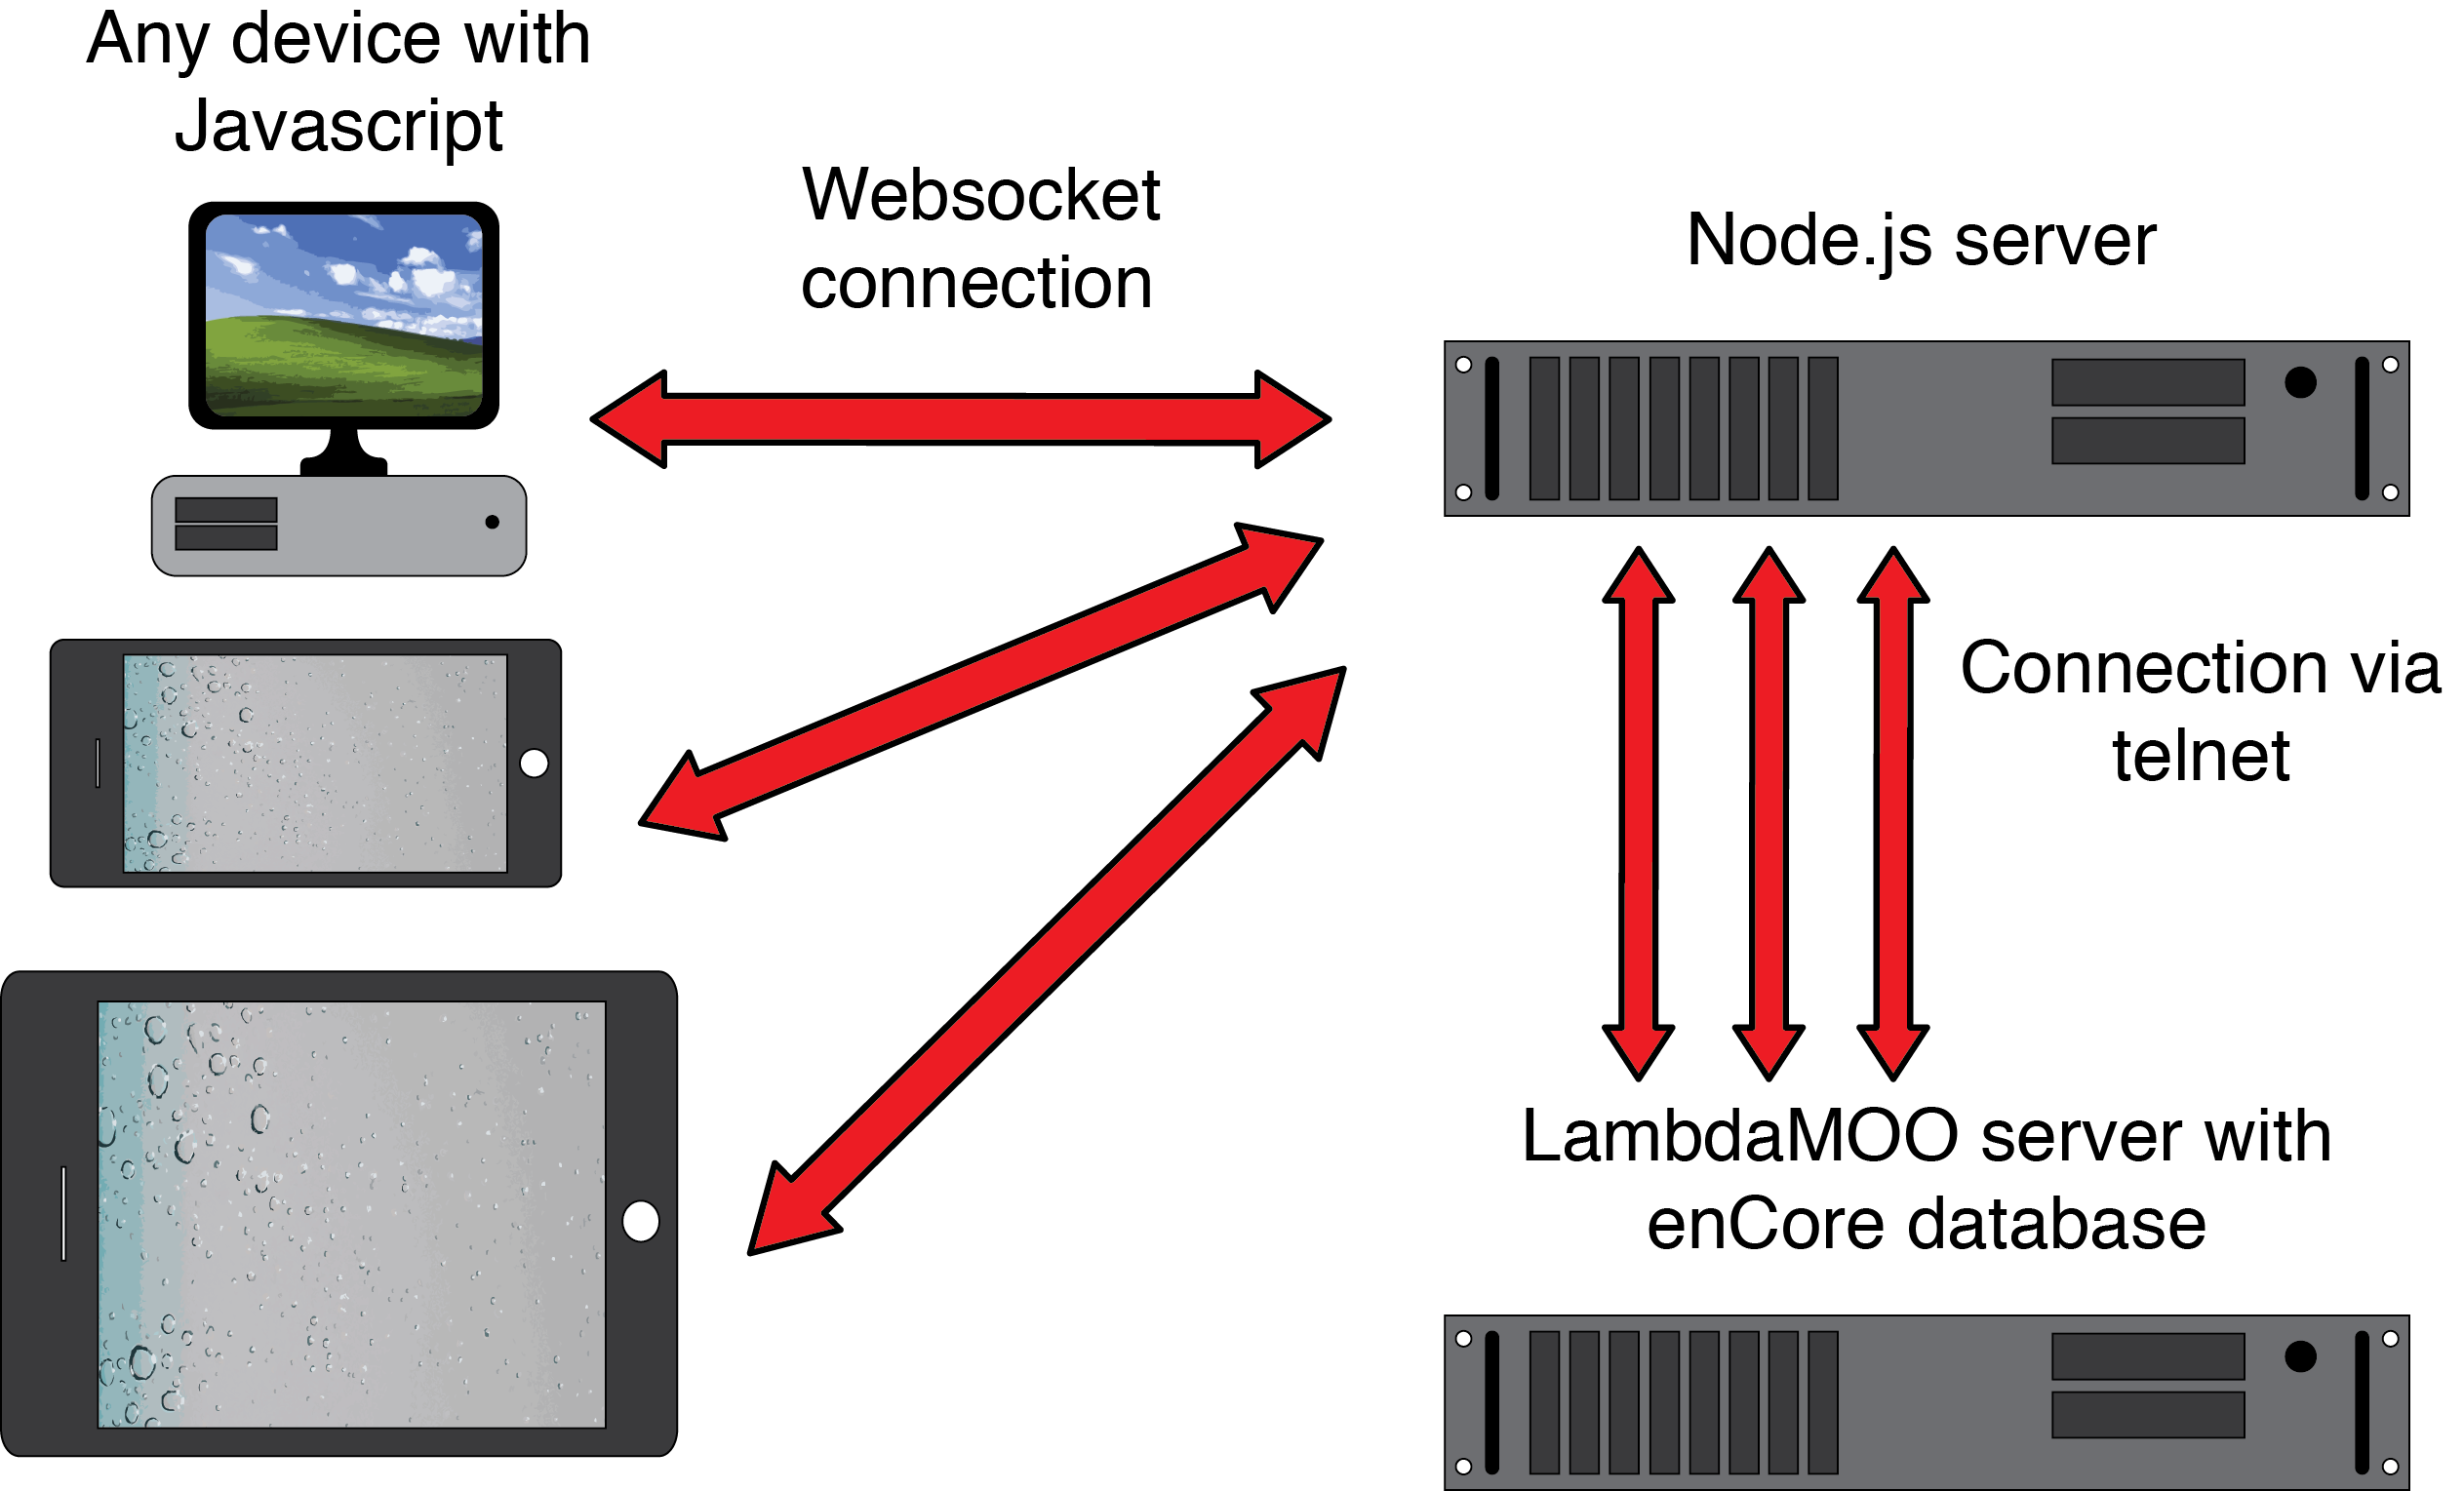
\includegraphics[width=\textwidth,height=\textheight,keepaspectratio]{NodeDiagram.png}
  \end{centering}
}

\section{Testing}
\frame{\frametitle{Testing}
  \begin{itemize}
    \item Unit Testing - Is a testing method where individual pieces of code or modules are tested in a controlled environment to make sure that the expected behaviour of the code occurs.
  \end{itemize}
}

\frame{\frametitle{Testing - Considerations}
  \begin{itemize}
    \item The structure of our code
    \begin{itemize}
      \item Our code is split up into different modules
    \end{itemize}
    \item The dependencies the code has
    \begin{itemize}
      \item RequireJs
      \begin{itemize}
        \item RequireJs is a modular script loader 
      \end{itemize}
      \item BackboneJs
      \begin{itemize}
        \item Backbone is what gives our code its structure, splitting it up into models, collections, and views
      \end{itemize}
    \end{itemize}
    \item What we want to do with it
    \begin{itemize}
    \item Continous Integration
    \end{itemize}
  \end{itemize}
}

\frame{\frametitle{Testing - Jasmine}
\begin{centering}

\includegraphics[width=0.2\textwidth, height=\textheight,keepaspectratio,center]{jasmine.png}
\begin{itemize}
\item Jasmine - A Behavior Driven Development testing framework for javascript
\item Pros
\begin{itemize}
  \item Simple setup for node through jasmine-node
  \item Large community, well supported with lots of documentation
  \item Nice fluent syntax for assertions built-in, and supports other assertion libraries
  \item Supported by many CI servers
  \item Descriptive syntax for BDD paradigm
\end{itemize}
\item Cons
\begin{itemize}
  \item Asynchronous testing can be a bit of a headache
\end{itemize}
\end{itemize}
\end{centering}
}

\section{Security}
\frame{\frametitle{Security}
  \begin{itemize}
    \item Telnet is plain text in transport, so it is inherently vulnerable to eavesdropping.
    \item For the initial work on the project, security is not a main concern.
    \item In the future, the telnet server can be protected from external network connections using containerization such as docker
    \item This way only the Node.js server can connect via telnet, and user data can be protected with SSL in transport.
    \item This strategy would disable the legacy enCore Xpress interface
  \end{itemize}
}
\section{Implementation}
\frame{\frametitle{New Client Text Interface}
  \begin{centering}
  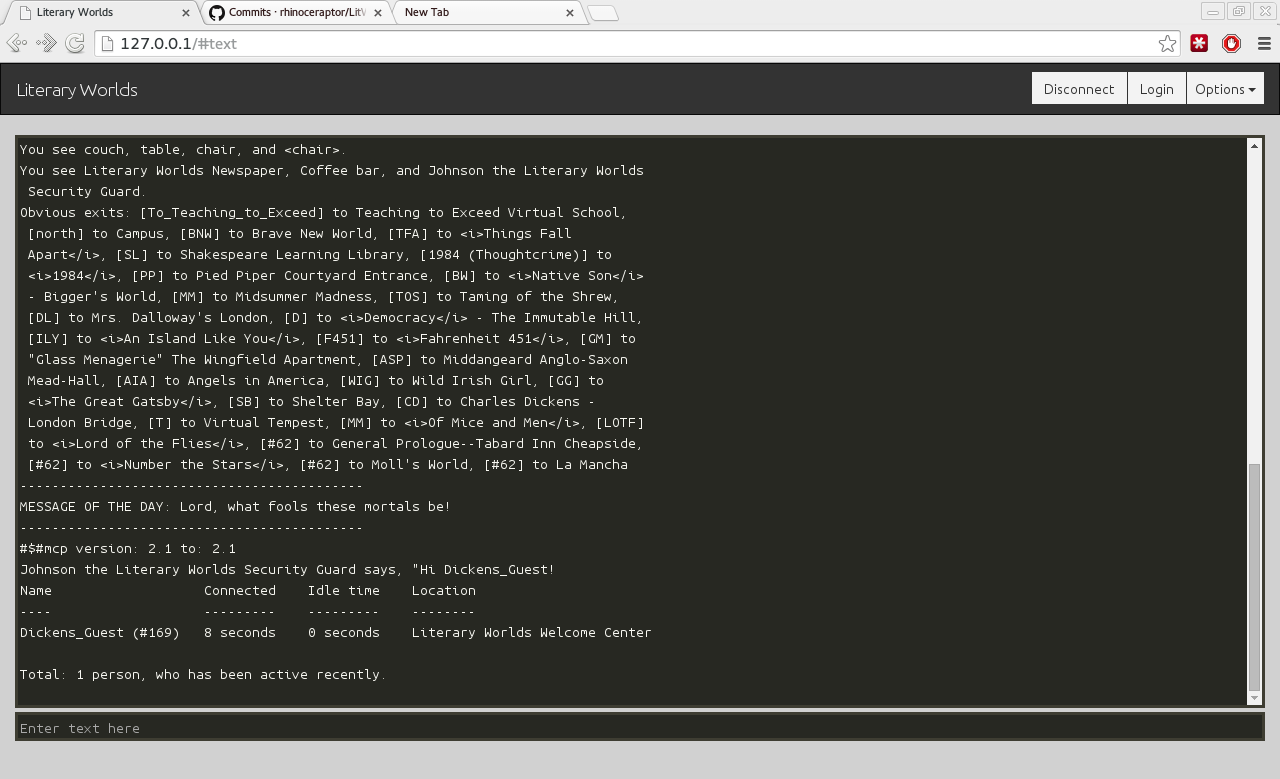
\includegraphics[width=\textwidth,height=\textheight,keepaspectratio]{litworlds_nov_28_text.png}
  \end{centering}
}


\frame{\frametitle{New Client Graphical Interface}
  \begin{centering}
  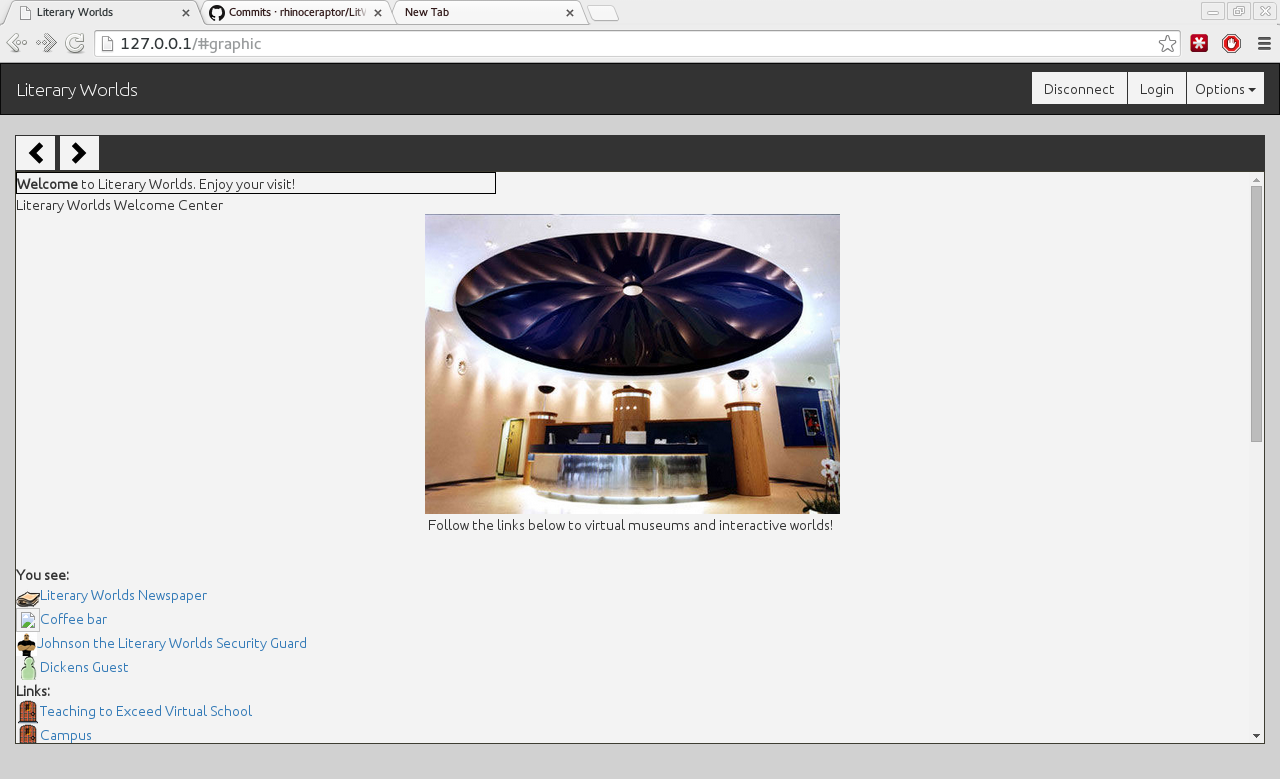
\includegraphics[width=\textwidth,height=\textheight,keepaspectratio]{litworlds_nov_28_graphic.png}
  \end{centering}
}


\frame{\frametitle{New Client Mixed Interface}
  \begin{centering}
  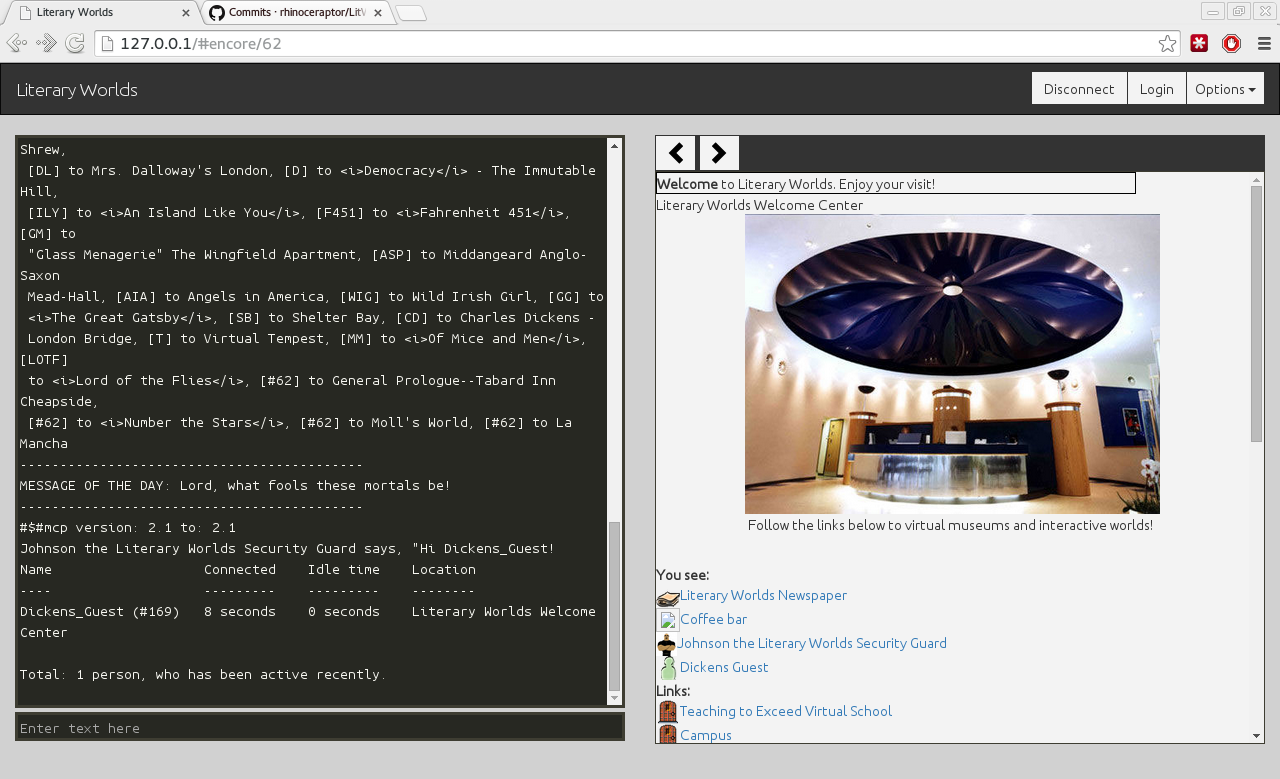
\includegraphics[width=\textwidth,height=\textheight,keepaspectratio]{litworlds_nov_28_mixed.png}
  \end{centering}
}

\frame{\frametitle{New Client Interface}
  \begin{centering}
    TBD - Repeat mixed mode example of getting pizza from the soma bar and Village example
  \end{centering}
}

\frame{\frametitle{Future of the New Client}
TBD - Who will get the code repo (likely Kevin)? Should mention we used Github for version control somewhere in presentation
Mention documentation and scripts we have writen???
Also mention future enchancements to back end...
}

\frame{\frametitle{Summary}
  \begin{itemize}
  \item Literary Worlds uses enCore Xpress to deliever text as well as other multimedia (music, picgtures, etc.) to users based on literary texts
  \item Used Backbone, Socket.io, Node.js, Express, and Bootstrap to create a new client interface
  \item Did not change the users experience or existing virtual worlds
  \item Successfully removed the need for Java and popups
  \end{itemize}
}

\frame{\frametitle{Questions}
\begin{centering}

\includegraphics[width=0.8\textwidth,height=0.8\textheight,keepaspectratio, center]{Help.png}
\end{centering}
}
\end{document}

